\documentclass[a4paper,10pt]{article}
\usepackage{booktabs}
\usepackage{graphicx}
\usepackage{etoolbox}
\usepackage{color}
\usepackage[hidelinks]{hyperref}

%-----------------------------------------------------------------------------

\hypersetup{
    colorlinks=false, %set true if you want colored links
    linktoc=all,     %set to all if you want both sections and subsections linked
    linkcolor=black,  %choose some color if you want links to stand out
}

%-----------------------------------------------------------------------------

\newtoggle{afterpart}
\pretocmd{\section}
  {\iftoggle{afterpart}
    {\global\togglefalse{afterpart}}% we're after a part
    {\clearpage}% we're not immediately after a part
  }{}{}
\pretocmd{\part}
  {\clearpage % do a page break
   \global\toggletrue{afterpart}% tell \section we're just after a part
  }
  {}{}

%-----------------------------------------------------------------------------

\title{SLIMER Update}
\author{Mary Kidd, Steve Elliott, Keith Rielage, Gwendolyn Buchanan}
\date{\today} % delete this line to display the current date

%-----------------------------------------------------------------------------

\begin{document}

\maketitle
\tableofcontents

\part{Eqipment Information}
\section{Objectives}

\begin{table}[!htbp]
	\centering
	\caption{Objectives}
	\vspace{.5cm}
	\label{tab:table2}
	\begin{tabular}{cccc}
		\toprule
		Objective & N. A. & Light Collection (\%) & $\phi$\\
		\midrule
		4X & 0.13 & 0.42 & ---\\
		10X & 0.30 & 2.3 & ---\\
		20X & 0.50 & 6.7 & ---\\
		40X & 0.75 & 16.9 & ---\\
		10XS & 0.50 & --- & 4.0\\
		20XS & 0.75 & --- & 4.0\\
		\bottomrule
	\end{tabular}
\end{table}

\section{Sources}

\begin{table}[!htbp]
	\centering
	\caption{Source list}
	\vspace{.5cm}
	\label{tab:table1}
	\begin{tabular}{ccccc}
		\toprule
		Source & Activity$_0$ & $t_0$ & $t_{1/2}$ & Activity$_t$\\
		\midrule
		$^{241}$Am $\alpha$ & 4.375 nCi & 01 Sept 2007 & 432.2 y & 4.313 nCi\\
		$^{241}$Am $\gamma$ & 10.51 $\mu$Ci & 12 Jan 1970 & 423.2 y & 9.75 $\mu$Ci\\
		$^{14}$C $\beta$ (strong) & 0.9853 $\mu$Ci & 15 Nov 2012 & 5730 y & 0.9849 $\mu$Ci\\
		$^{14}$C $\beta$ (weak) & 45.18 nCi & 01 Sept 2011 & 5730 y & 45.15 nCi\\
		$^{133}$Ba $\gamma$ & 9.907 $\mu$Ci & 01 Oct 2003 & 10.51 y & 4.263 $\mu$Ci\\
		$^{137}$Cs (window) & 10 $\mu$Ci & 01 Oct 2003 & 30.07 y & 2.4 $\mu$Ci\\
		$^{90}$Sr & 31.35 $\mu$Ci & 20 July 1981 & 28.78 y & 13.47 $\mu$Ci\\ 
		$^{22}$Na & 9.030 $\mu$Ci & 01 Oct 2003 & 2.6019 y & 0.299 $\mu$Ci\\
		\bottomrule
	\end{tabular}
\end{table}

%-----------------------------------------------------------------------------

\part{Data}
\section{$^{241}$Am $\alpha$}

$^{241}$Am alphas have energies of 5442.80 keV (13.1\%) and 5485.56 keV (84.8\%).

\subsection{Example Event}
\begin{figure}[!htbp]
   \centering
   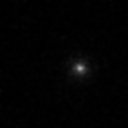
\includegraphics[width=3in,keepaspectratio]{241Am-alpha_example.jpg} % requires the graphicx package
   \caption{$^{241}$Am alpha event with 10XS objective and 4x4 binning.}
   \label{fig:10XSAmalpha}
\end{figure}

\subsection{Peak Height Data}
\begin{figure}[!htbp]
	\centering
	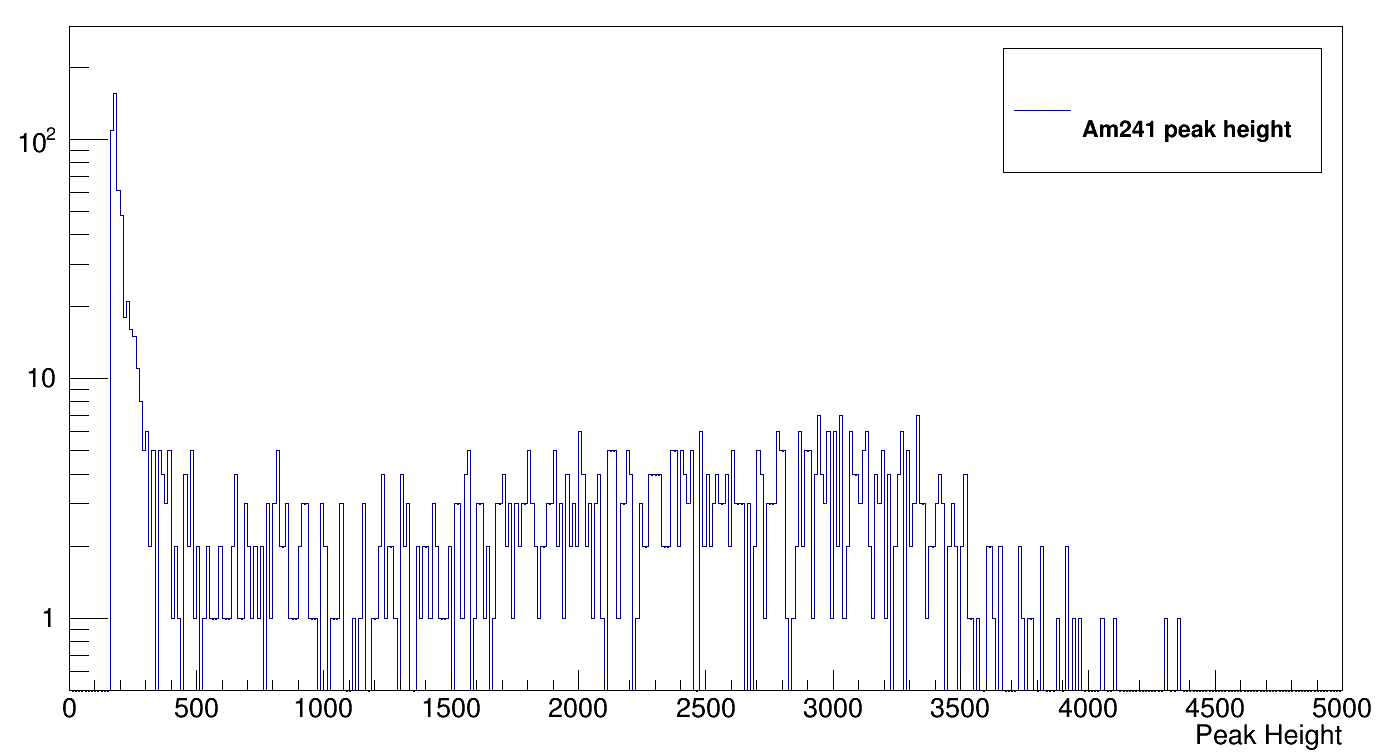
\includegraphics[width=3.2in,keepaspectratio]{Am-alpha-peakheight.png}
	\caption{$^{241}$Am alpha peak heights, Run 081. Includes gammas.}
	\label{fig:Am-allpha-peakheights}
\end{figure}

\section{$^{241}$Am $\gamma$}

$^{241}$Am gammas have energies of 13.9 keV (37\%) and 59.5409 keV (35.9\%).

\subsection{Example Event}
\begin{figure}[!htbp]
	\centering
	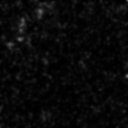
\includegraphics[width=3in,keepaspectratio]{241Am-gamma_example.jpg}
	\caption{$^{241}$Am gamma event with 10XS objective and 4x4 binning. Gamma events are present in the alpha $^{241}$Am source, but are adjusted into the background because of the brightness of the alpha events.}
	\label{fig:10XSAmgamma}
\end{figure}

\subsection{Peak Height Data}
\begin{figure}[!htbp]
	\centering
	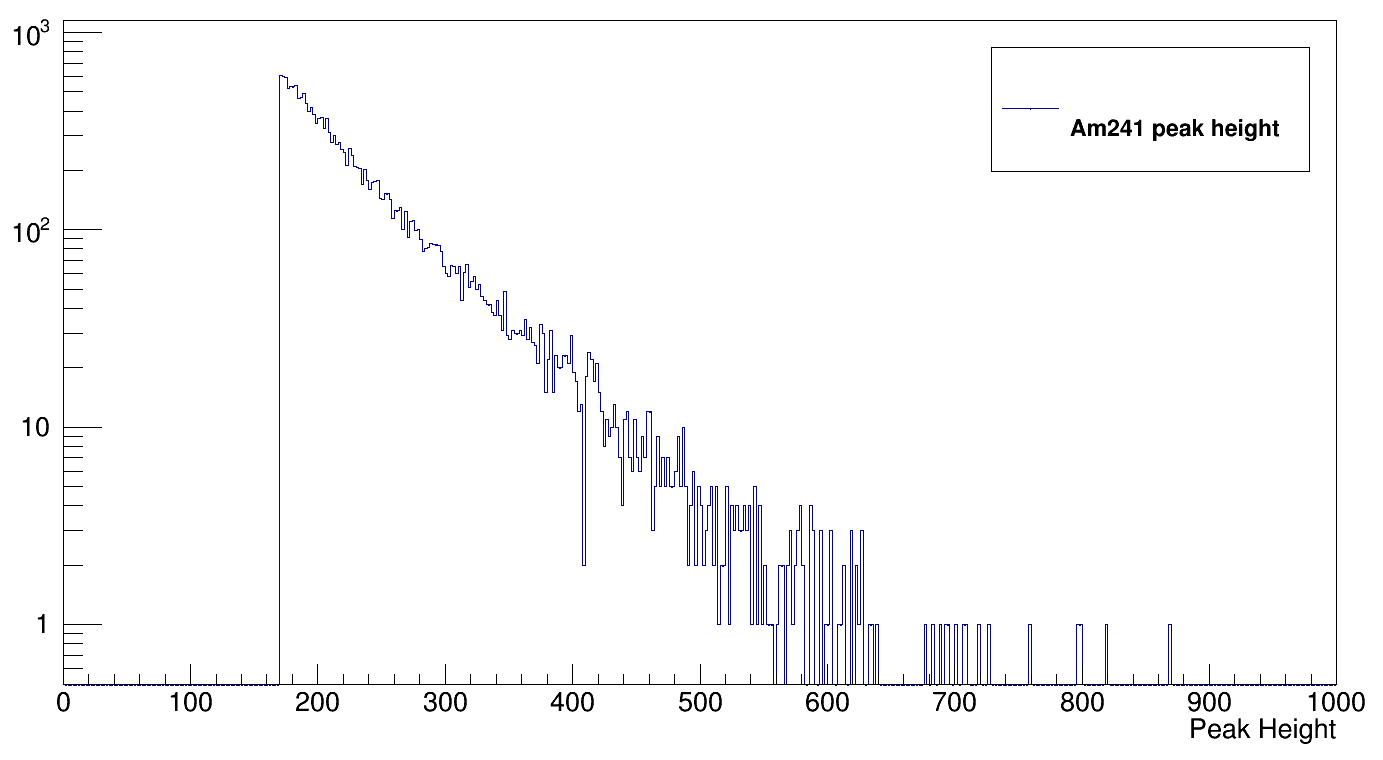
\includegraphics[width=3.2in,keepaspectratio]{Am-peakheight.png}
	\caption{$^{241}$Am gamma peak heights, from Run 034. No alpha events.}
	\label{fig:Am-gamma-peakheights}
\end{figure}

\section{$^{14}$C $\beta$ (strong)}

$^{14}$C betas have an energy spectrum with a mean of 49.47 keV and an endpoint of 156.475 keV.

\subsection{Example Event}
\begin{figure}[!htbp]
	\centering
	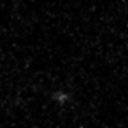
\includegraphics[width=3in,keepaspectratio]{14Cstrong-beta_example.jpg}
	\caption{Beta event in the strong $^{14}$C source with 10XS objective and 4x4 binning.}
	\label{fig:10XSCstrongbeta}
\end{figure}

\subsection{Peak Height Data}
\begin{figure}[!htbp]
	\centering
	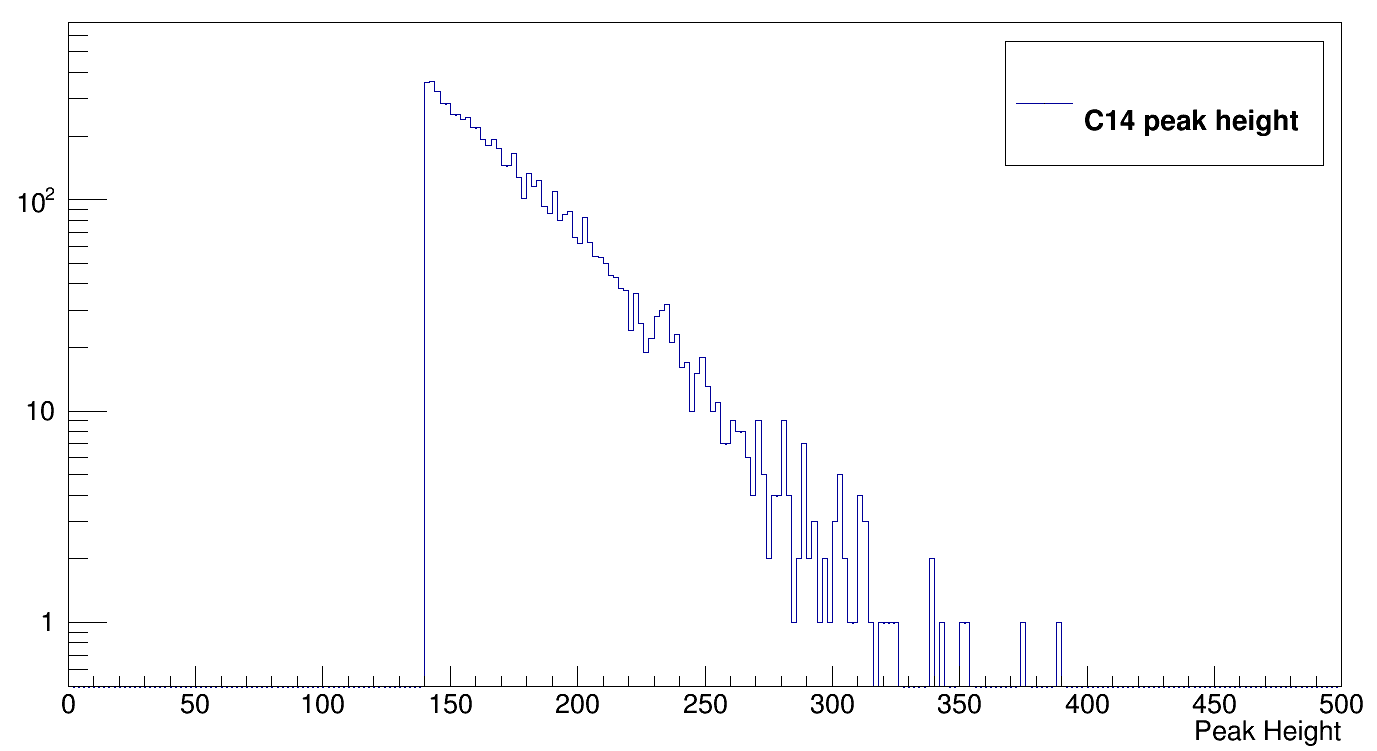
\includegraphics[width=3.2in,keepaspectratio]{C14-peakheight.png}
	\caption{$^{14}$C peak heights taken from Run 067, using the strong $^{14}$C source.}
	\label{fig:C-peakheights}
\end{figure}

\section{$^{14}$C $\beta$ (weak)}

$^{14}$C betas have an energy spectrum with a mean of 49.47 keV and an endpoint of 156.475 keV.

\subsection{Example Event}
\begin{figure}[!htbp]
	\centering
	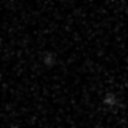
\includegraphics[width=3in,keepaspectratio]{14Cweak-beta_example.jpg}
	\caption{Beta event in the weak $^{14}$C source with 10XS objective and 4x4 binning.}
	\label{fig:10XScweakbeta}
\end{figure}

\subsection{Peak Height Data}
\begin{figure}[!htbp]
	\centering
	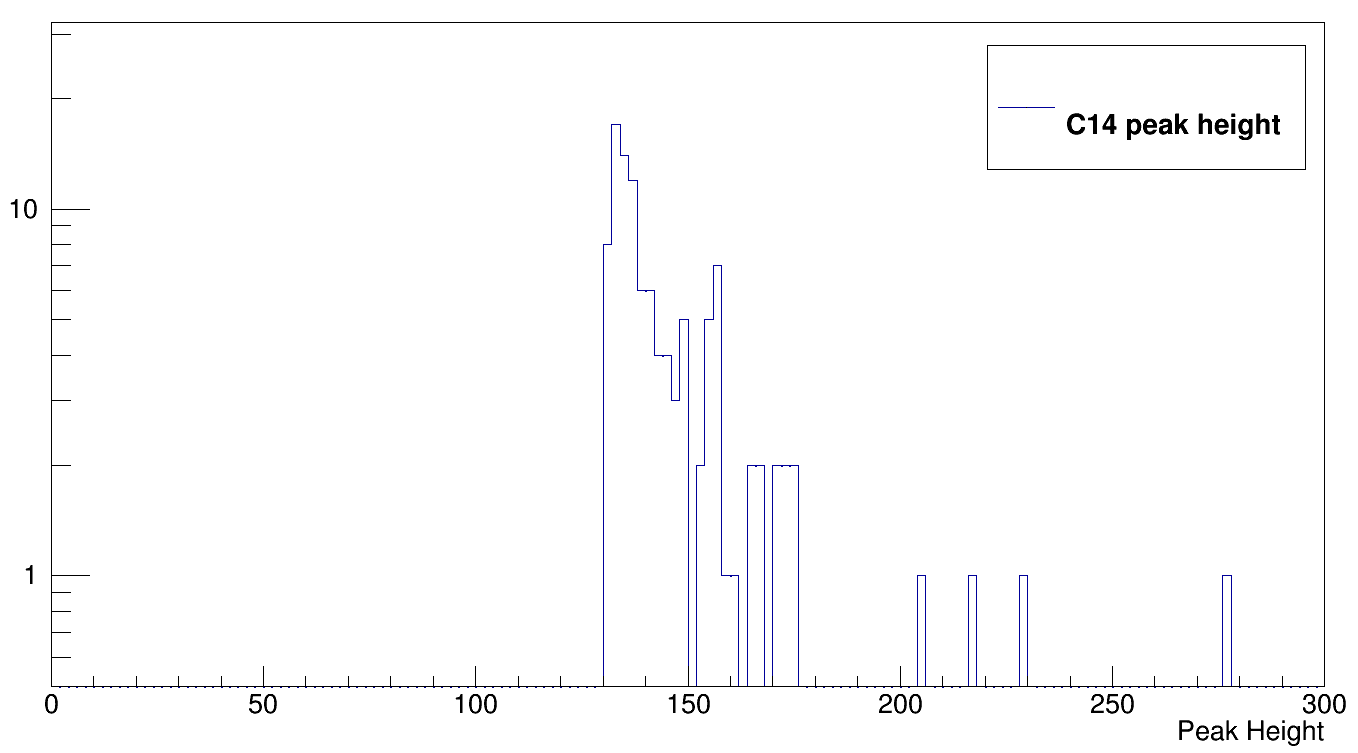
\includegraphics[width=3.2in,keepaspectratio]{C14-weak-peakheight.png}
	\caption{Peak heights from Run 049 with the weak $^{14}$C source.}
	\label{fig:C-weak-peakheights}
\end{figure}

\section{$^{133}$Ba $\gamma$}

$^{133}$Ba gammas have energies of 4.47 keV (16.4\%), 31.817 keV (15.1\%), 32.194 keV (27.6\%), and 275.925 keV (17.69\%).

\subsection{Example Event}
\begin{figure}[!htbp]
	\centering
	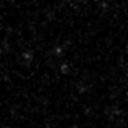
\includegraphics[width=3in,keepaspectratio]{133Ba-gamma_example.jpg}
	\caption{Ba gamma event with 10XS objective and 4x4 binning.}
	\label{fig:10XSBagamma}
\end{figure}

\subsection{Peak Height Data}
\begin{figure}[!htbp]
	\centering
	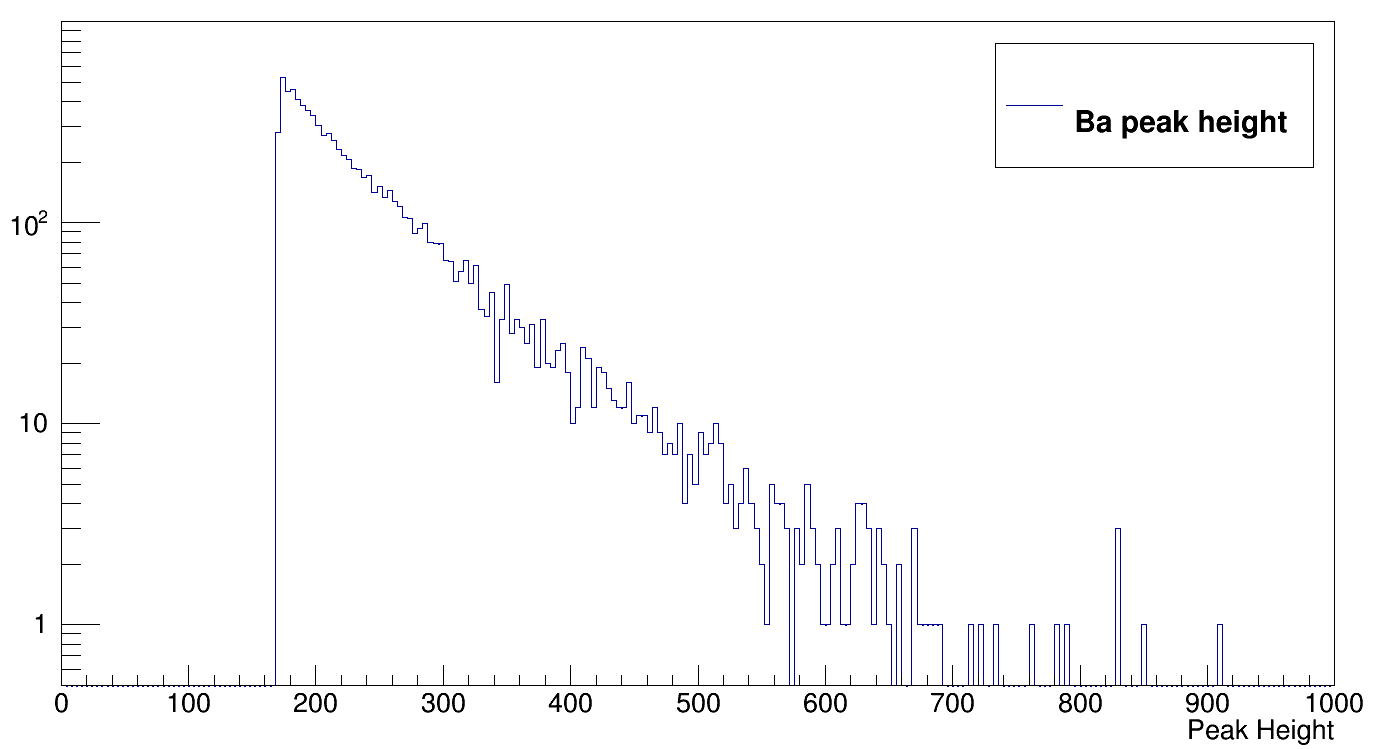
\includegraphics[width=3.2in,keepaspectratio]{Ba-peakheight.png}
	\caption{$^{133}$Ba peak heights from Run 032.}
	\label{fig:Ba-peakheight}
\end{figure}

\section{$^{137}$Cs (window)}

$^{137}$Cs betas have an energy of 174.32 keV (94.70\%) with an endpoint of 513.97 keV. $^{137}$Cs gammas have an energy of 661.657 keV (85.10\%).

\subsection{Example Event}
\begin{figure}[!htbp]
	\centering
	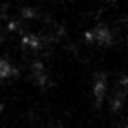
\includegraphics[width=3in,keepaspectratio]{137Cs-beta_example.jpg}
	\caption{Gamma and beta events with 10XS objective and 4x4 binning.}
	\label{fig:10XSCsbeta}
\end{figure} 

\subsection{Peak Height Data}
\begin{figure}[!htbp]
	\centering
	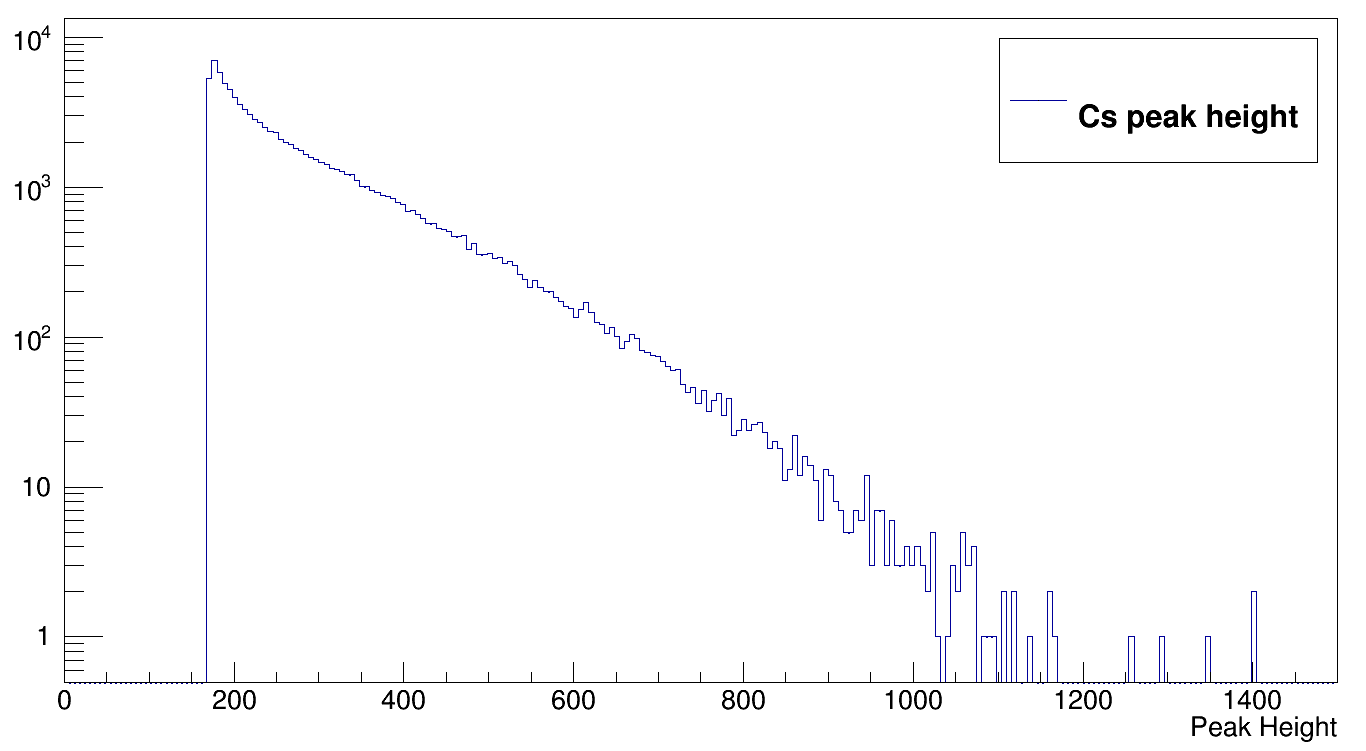
\includegraphics[width=3.2in,keepaspectratio]{Cs-peakheight.png}
	\caption{Peak heights of $^{137}$Cs from Run 036.}
	\label{fig:Cs-peakheight}
\end{figure}

\section{$^{90}$Sr}

$^{90}$Sr betas have an energy spectrum with a mean of 195.8 keV and an endpoint of 546.0 keV.

\subsection{Example Event}
\begin{figure}[!htbp]
	\centering
	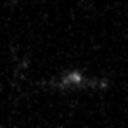
\includegraphics[width=3in,keepaspectratio]{90Sr-beta_example.jpg}
	\caption{Sr beta event with 10XS objective and 4x4 binning.}
	\label{fig:10XSSrbeta}
\end{figure}

\subsection{Peak Height Data}
\begin{figure}[!htbp]
	\centering
	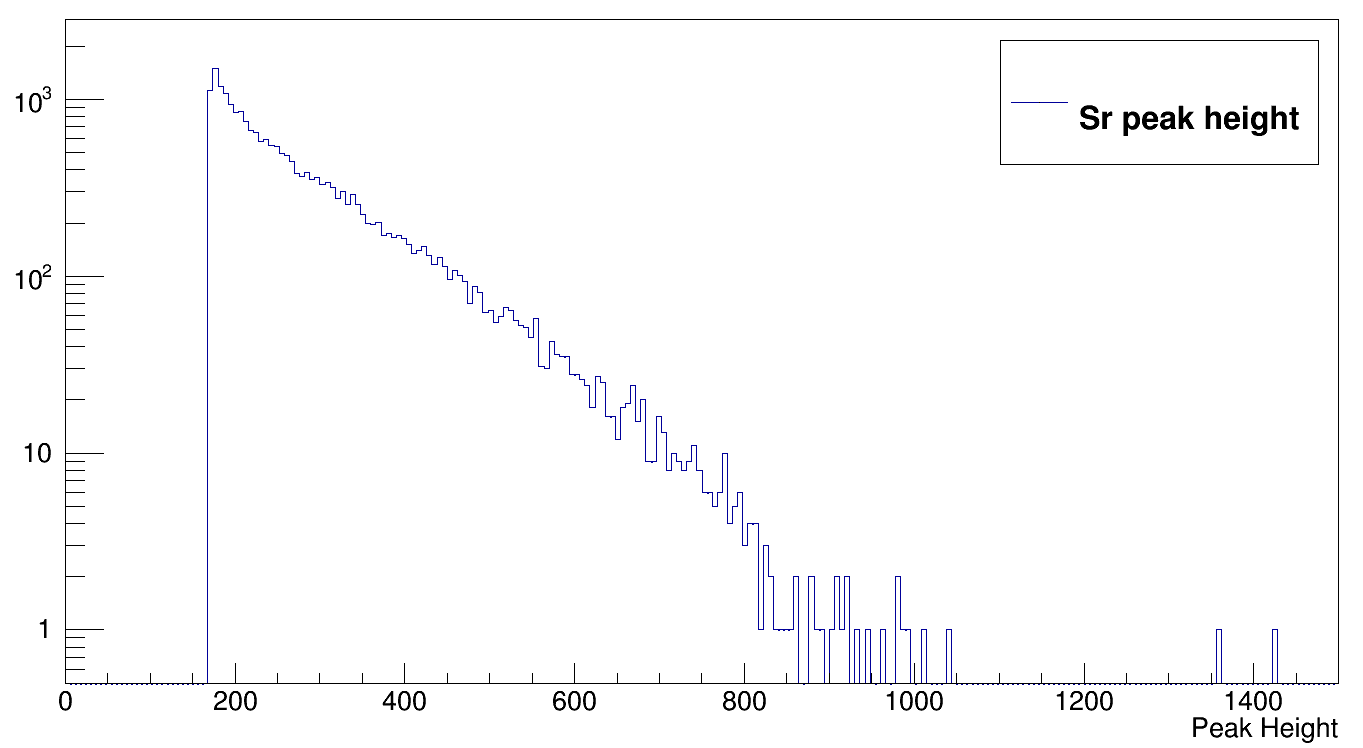
\includegraphics[width=3.2in,keepaspectratio]{Sr-peakheight.png}
	\caption{Peak heights of $^{90}$Sr from Run 021.}
	\label{fig:Sr-peakheight}
\end{figure}

%-----------------------------------------------------------------------------

\part{Simulation}
\section{Structure and Running}

\subsection{Structure}

The DetectorConstruction file generates the physical objects associated with the simulation: the CsI cylinders, the objective lens, and so on. RunAction oversees the whole run, while EventAction and SteppingAction handle events and steps, respectively. A run consists of events, which consist of steps. TrackingAction tracks particles. PhysicsList gets the necessary physics processes. PrimaryGeneratorAction creates the particle source. 

The exec.mac macro sets up the geometry of the detector, while run.mac actually creates particles. Particle location, energy, and type, along with number of runs, are changed in run.mac. CMakeLists.txt is used for making the executable and should not be changed. The executable, exec.cc, should also not be changed. 

\subsection{Running}

Required software: 

\begin{itemize}
	\item Geant4 9.6, patch 04
	\item CMake 2.8.12 or higher
	\item ROOT 5.34/14
\end{itemize}

The primary directory is called \textit{code}, and contains directories labeled \textit{include}, \textit{misc}, and \textit{src} along with files CMakeLists.txt, exec.cc, exec.mac, run.mac, and README.md.

\subsubsection{Compiling and running on Ubuntu 12.04} 

\begin{itemize}
	\item Create a directory \textit{code\_build} parallel to \textit{code}.
	\item In a terminal, navigate to the \textit{code\_build} directory. 
	\item From \textit{code\_build}, run \texttt{ \# cmake -DGeant4\_DIR=/path/to/\\geant4.9.6.p04/lib[64]/Geant4-9.6.0/ ../code/ }.
	\item Run \texttt{ \# make \&\& make install }.
	\item Run \texttt{ \# ./exec exec.mac }to set up the geometry.
	\item Run \texttt{ \# ./exec run.mac } to run the events and generate the .root file.
\end{itemize}


\subsubsection{Compiling and running on Mac OS X}

\begin{itemize}
	\item Create a directory \textit{code\_build} parallel to \textit{code}.
	\item In a terminal, navigate to the \textit{code\_build} directory. 
	\item From \textit{code\_build}, run \texttt{ \# cmake -DGeant4\_DIR=/path/to/\\geant4.9.6.p04/build ../code/ }.
	\item Run \texttt{ \# make \&\& make install }.
	\item Run \texttt{ \# ./exec exec.mac }to set up the geometry.
	\item Run \texttt{ \# ./exec run.mac } to run the events and generate the .root file.
\end{itemize}

\section{Simulated Spectra}

\subsection{Simulated $^{14}$C}

\begin{figure}[!htbp]
	\centering
	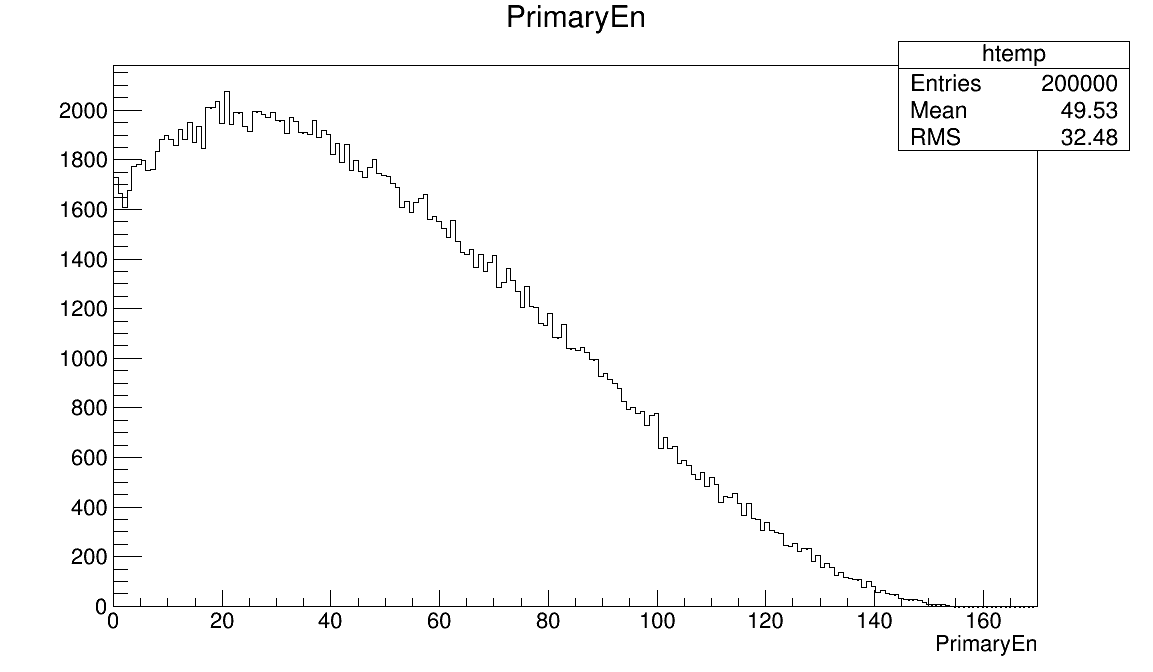
\includegraphics[width=4.5in,keepaspectratio]{C-simulated.png}
	\caption{$^{14}$C simulated spectrum.}
	\label{fig:14Csim}
\end{figure}

\subsection{Simulated $^{137}$Cs}

\begin{figure}[!htbp]
	\centering
	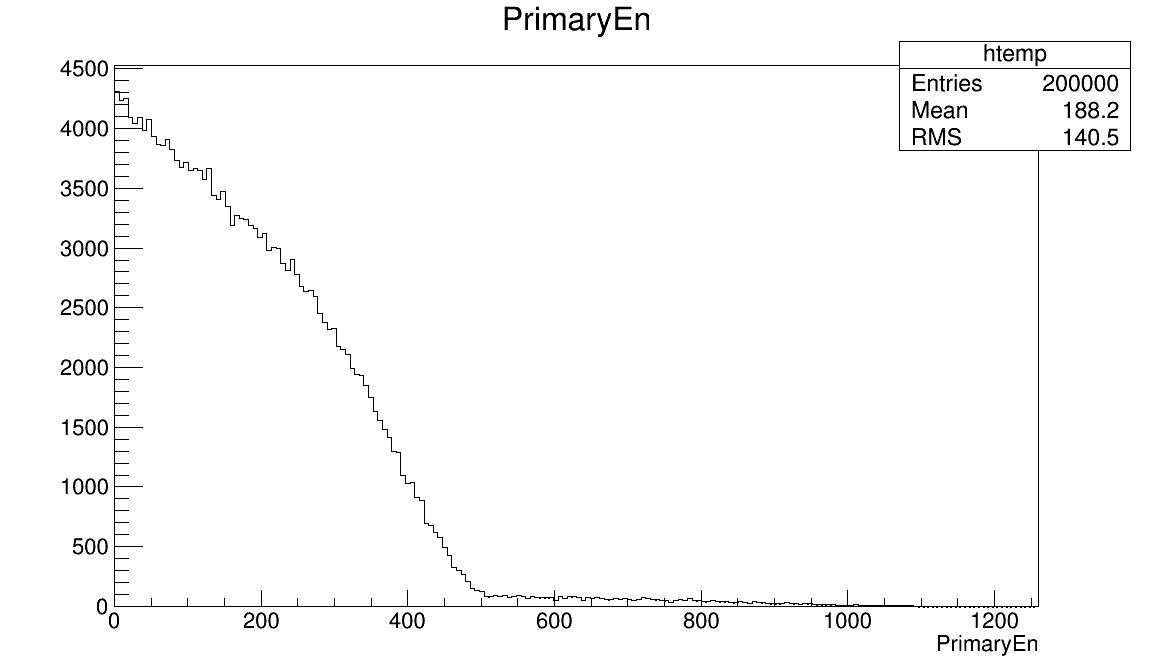
\includegraphics[width=4.5in,keepaspectratio]{Cs-simulated.png}
	\caption{$^{137}$Cs simulated spectrum.}
	\label{fig:Amsim}
\end{figure}

\subsection{Simulated $^{90}$Sr with $^{90}$Y}

\begin{figure}[!htbp]
	\centering
	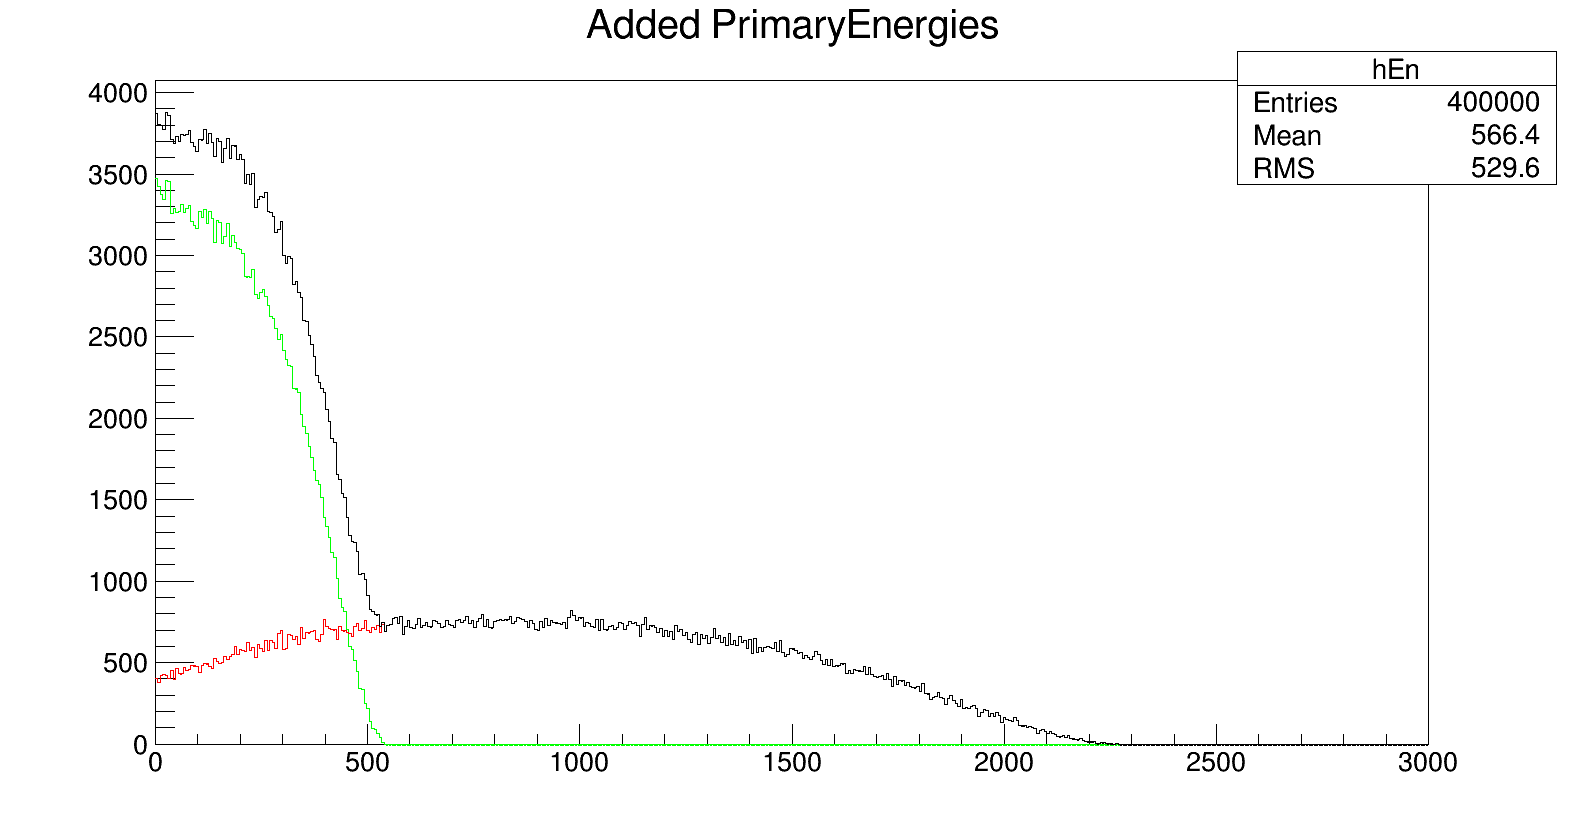
\includegraphics[width=4.5in,keepaspectratio]{Added-simulated.png}
	\caption{$^{90}$Sr and Y simulated spectrum.}
	\label{fig:SrYsim}
\end{figure}

%-----------------------------------------------------------------------------

\part{Simulation/Data Comparison}

The real data is calibrated to the simulation data in order to give the simulation data units. The peak height data from ImageJ can be compared to the energy absorbed data from the simulation. 

\section{Calibration Procedure}

For each value in the Max histogram (which contains the peak height data), a calibrated value is produced using the formula maxcal = $b*$max$+a$. The parameters $a$ and $b$ come from a graph of eAbs vs. gray value (see Figure \ref{fig:calgraphs}), where eAbs is the energy absorbed data from the simulation and gray value is the peak height data from ImageJ. The values used here come from C, Cs, and Sr.

\begin{figure}[!htbp]
	\centering
	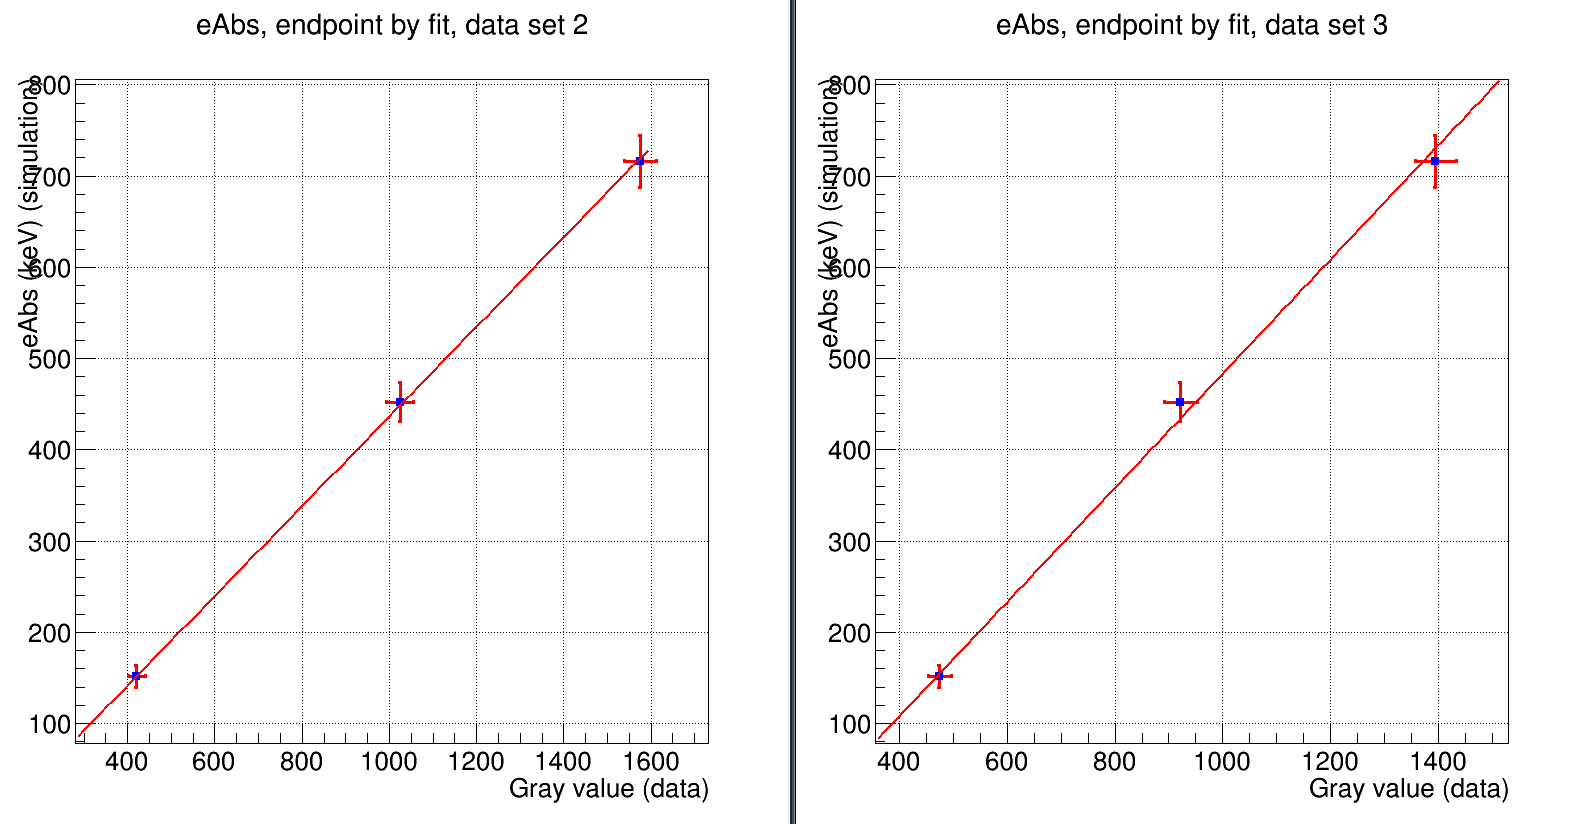
\includegraphics[width=4.5in,keepaspectratio]{calgraphs.png}
	\caption{Left: $f(x) = 0.49x-55$. Right: $f(x) = 0.63x-141.83$.}
	\label{fig:calgraphs}
\end{figure}

\section{Issues with Calibration}

The first main issue with calibration is that different sets of C, Cs, and Sr data do not produce the same line. The two sets of data in Figure \ref{fig:calgraphs} were taken under conditions as identical as possible, within minutes of each other, but produce very different parameters. 

The second issue with calibration is that the same values for $a$ and $b$ do not produce the same results for two isotopes. Both sets of data in Figure \ref{fig:different} were calibrated using the second set of parameters from Figure \ref{fig:calgraphs}.

\begin{figure}[!htbp]
	\centering
	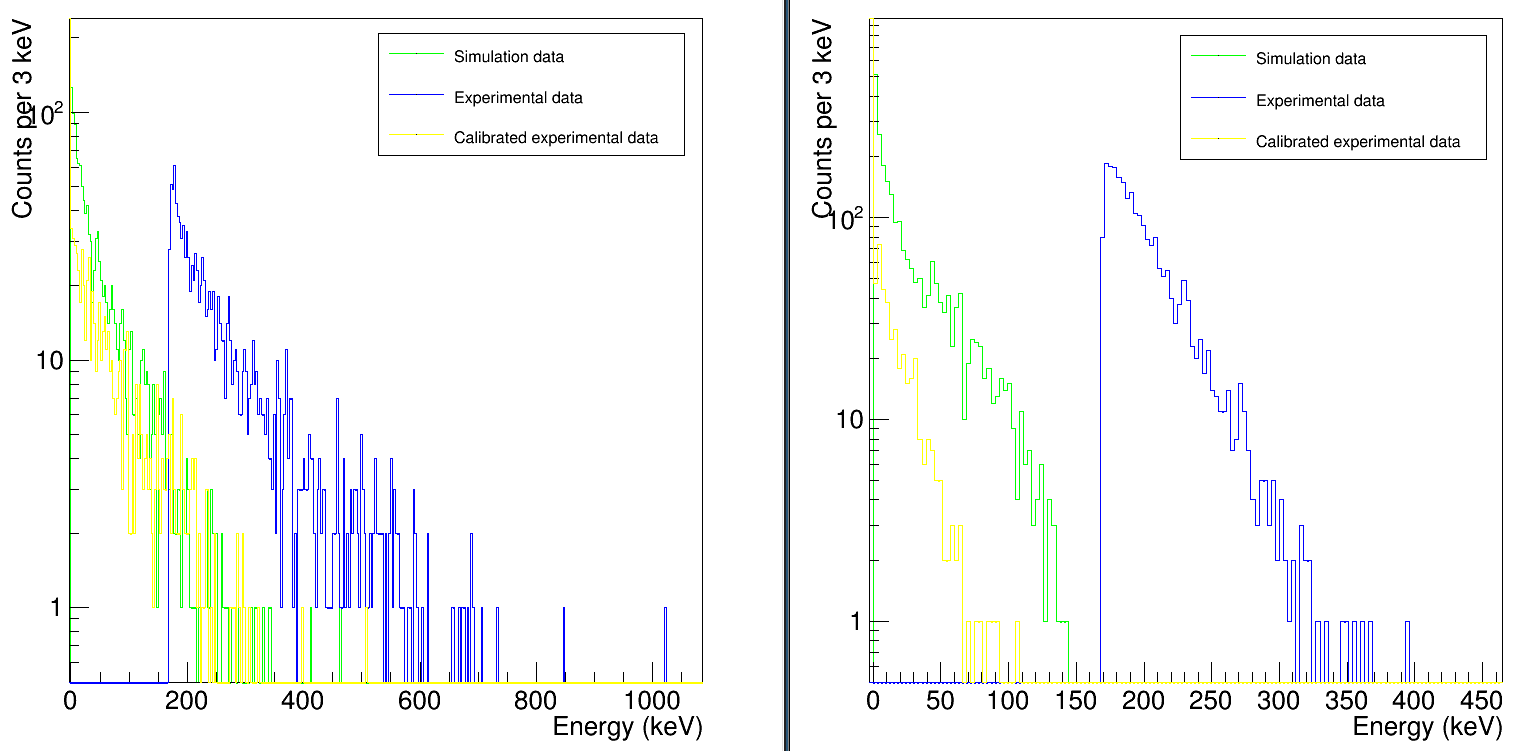
\includegraphics[width=4.5in,keepaspectratio]{different.png}
	\caption{Left: $^{137}$Cs, $\chi ^2$/ndf = 1.39. Right: $^{14}$C, $\chi ^2$/ndf = 3.30.}
	\label{fig:different}
\end{figure}

%-----------------------------------------------------------------------------

\part{Minimum Detectable Activity}

To get an idea of the minimum activity detectable in 10,000 images, runs were taken with several activity levels of $^{14}$C and $^{241}$Am. This was achieved by masking the available $^{14}$C and $^{241}$Am sources with two different sizes of colimators: 250 $\mu$m and 1 mm. The lower-activity of the two available $^{14}$C sources was not masked, because of its already low activity. 

The EventFinder macro, which sorts images into those with events and those without, usually picks up about 250 images as having events even though they do not. Therefore, the y-intercept of these graphs is around 250. 

\begin{figure}[!htbp]
	\centering
	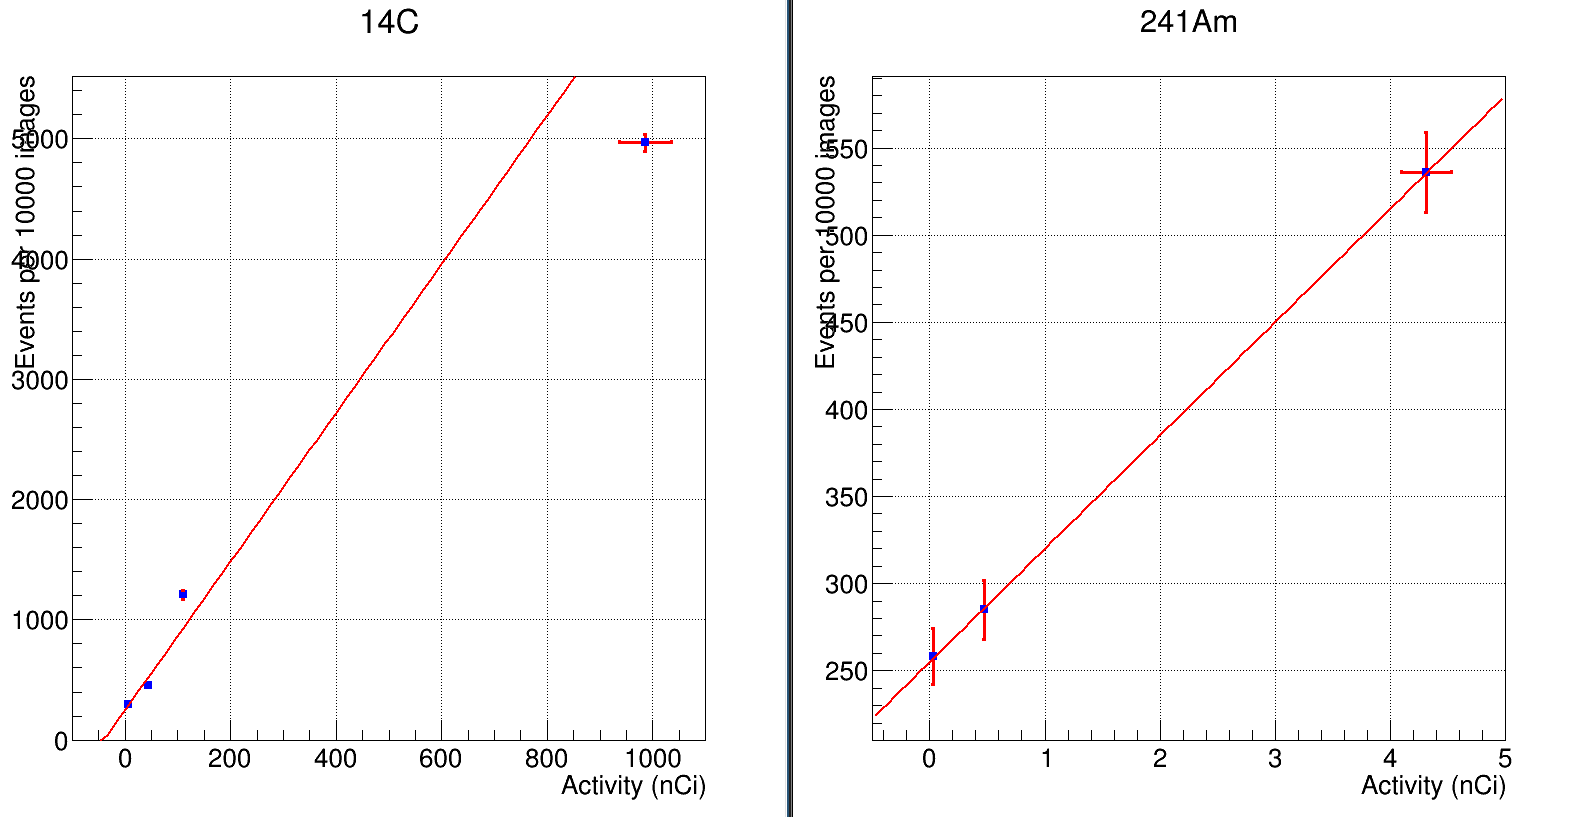
\includegraphics[width=4.5in,keepaspectratio]{min_activity.png}
	\caption{Graph of number of events vs. activity.}
	\label{fig:mindetect}
\end{figure}

%-----------------------------------------------------------------------------

\part{Position Resolution}

\section{Data Analysis}

Runs were taken using a 1 mm colimator. However, because 1 mm is almost as large as the field of view with the 10XS objective, the colimator was positioned so that only half of it was in the field of view.

\begin{figure}[!htbp]
	\centering
	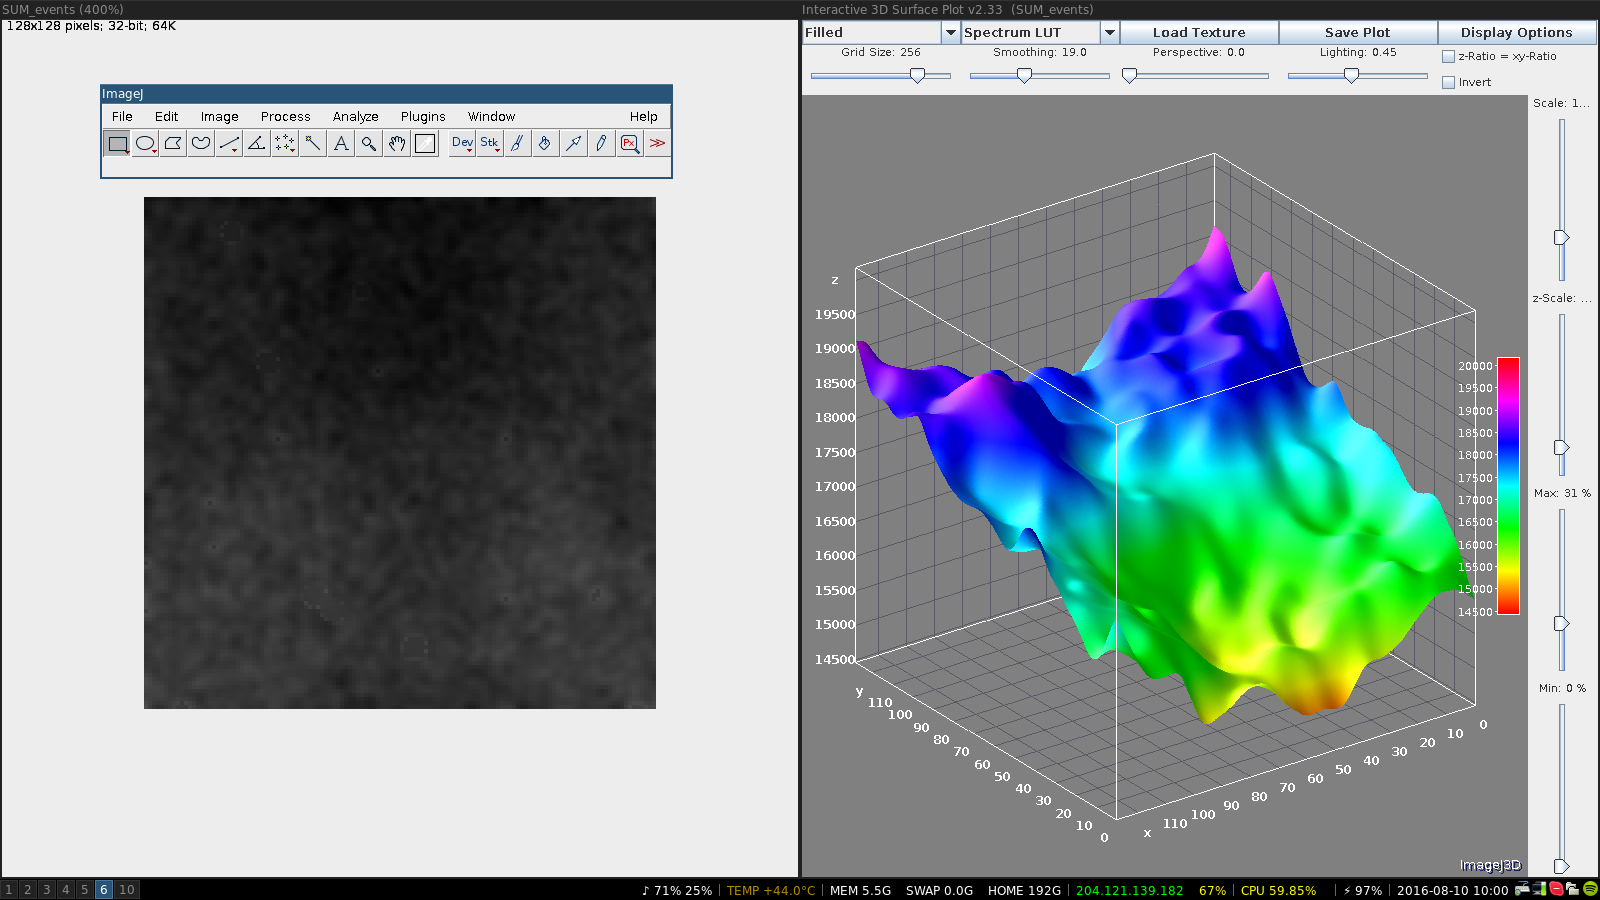
\includegraphics[width=4.5in,keepaspectratio]{3dplot.png}
	\caption{$^{14}$C run and 3D plot. Notice that although (0,0) in the image is at the upper left corner, (0,0) in the 3D plot is at the lower right corner.}
	\label{fig:3dplot}
\end{figure}

\begin{figure}[!htbp]
	\centering
	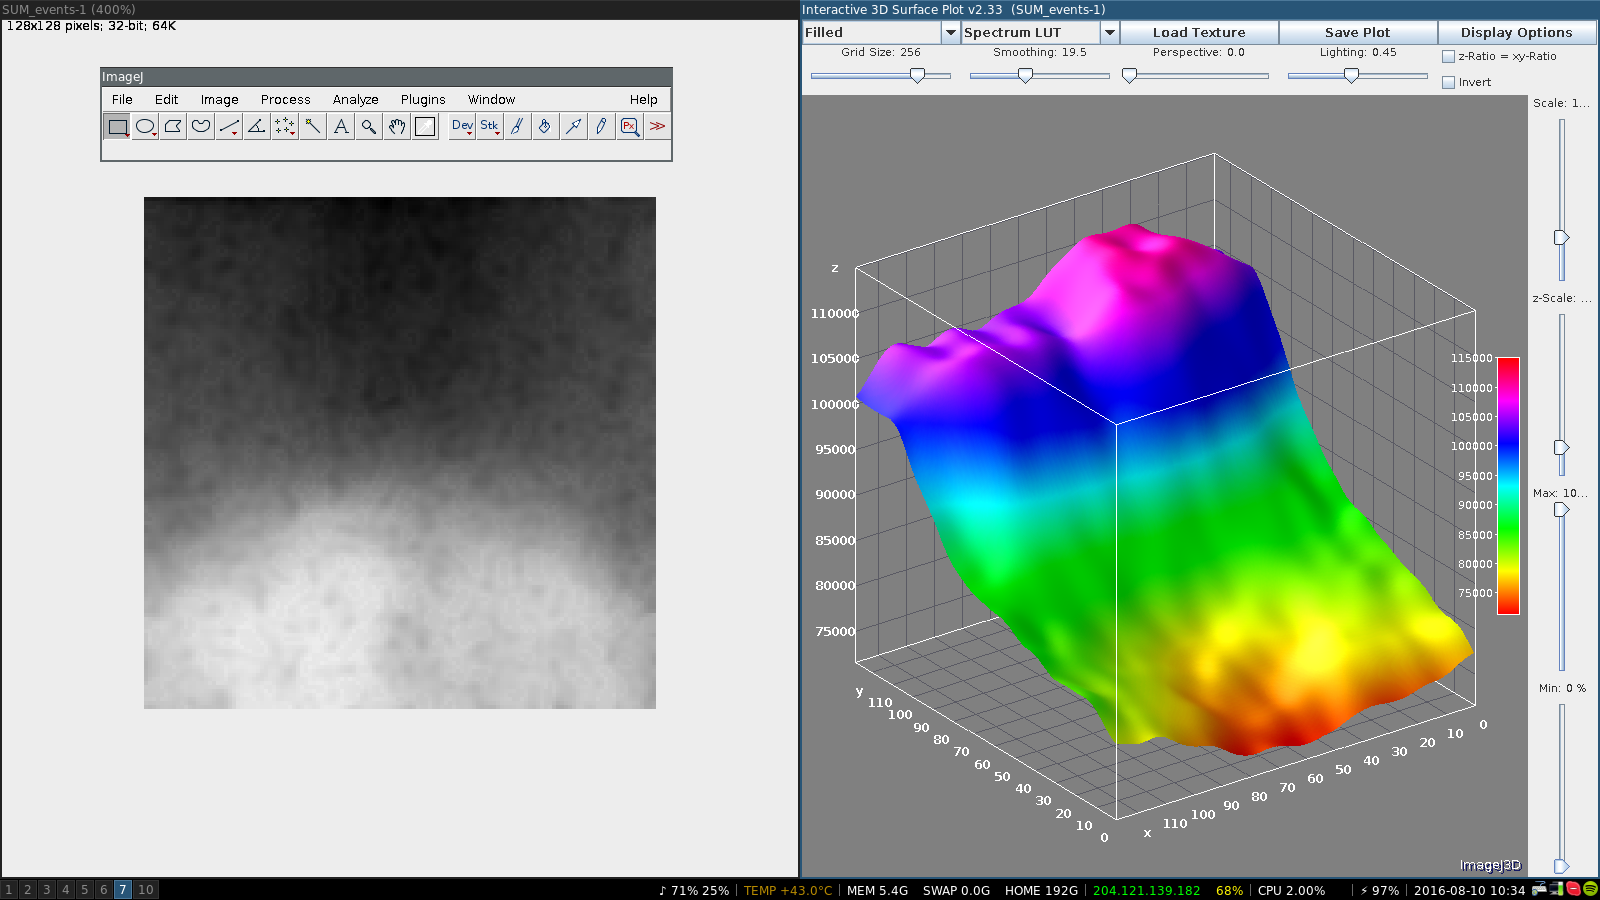
\includegraphics[width=4.5in,keepaspectratio]{3dplotSr.png}
	\caption{$^{90}$Sr run and 3D plot. Again, (0,0) in the image is at the upper left corner, and (0,0) in the 3D plot is at the lower right corner.}
	\label{fig:3dplotSr}
\end{figure}

\section{Determining Resolution}

Ideally, looking at a sideview of the plots would give a clear estimate of the horizontal distance, in pixels, from the top (unmasked area) to the bottom (masked area). 

\begin{figure}[!htbp]
	\centering
	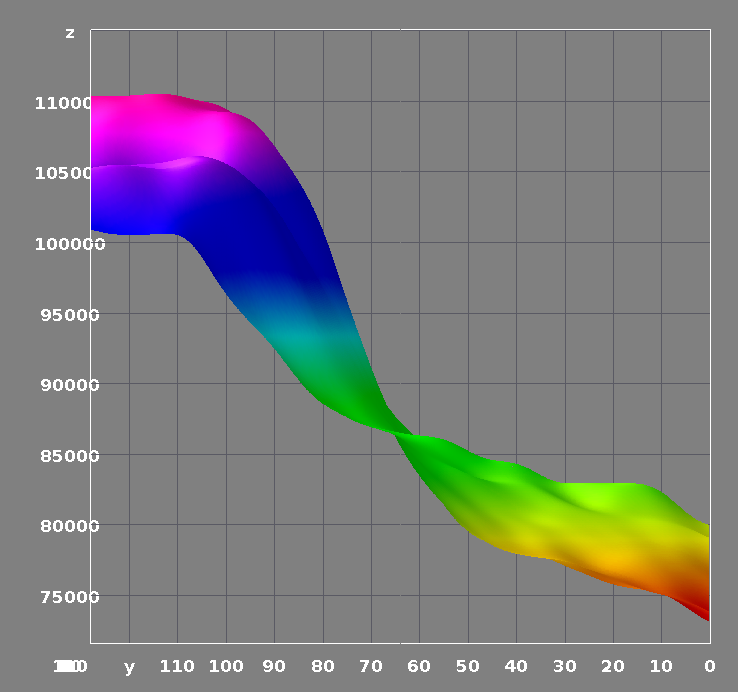
\includegraphics[width=2.2in,keepaspectratio]{3d_sideview_Sr.png}
	\hspace{0.1in}
	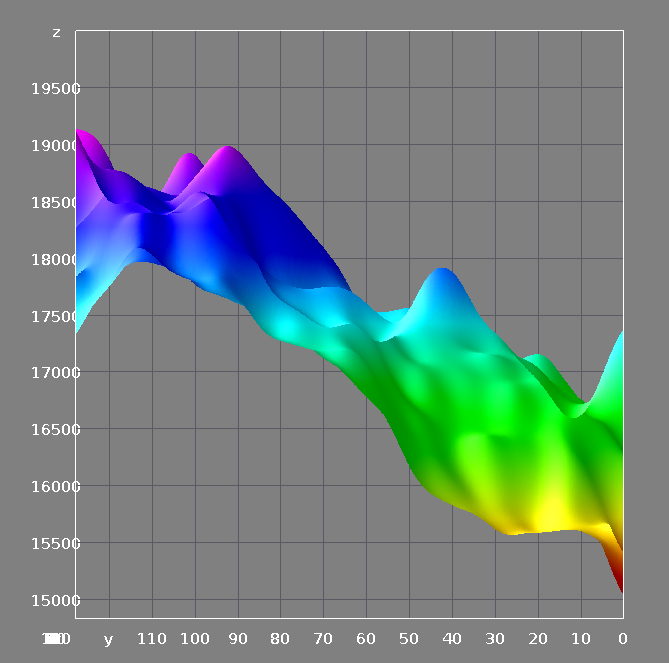
\includegraphics[width=2.2in,keepaspectratio]{3d_sideview_C14.png}
	\caption{Left: $^{90}$Sr. Right: $^{14}$C.}
	\label{fig:sideviews}
\end{figure}

A reasonable estimate might be 50 pixels for $^{90}$Sr and 80 pixels for $^{14}$C. The image is 128x128 pixels, corresponding to 0.707x0.707 mm. Thus, the position resolution for $^{90}$Sr is around 0.28 mm, and for $^{14}$C is around 0.44 mm.

%-----------------------------------------------------------------------------

\part{List of Macros}
\section{ImageJ Macros}

\subsection{getAverage}

getAverage gets the average of all the images in the run. It can be run with up to 25000 images at once. 

\subsection{subtractAverage}

subtractAverage subtracts the average generated with getAverage from every image. It can be run with up to 3000 images at once.

\subsection{gaussianBlur}

guassianBlur runs ImageJ's Gaussian Blur function on every image. It can be run with up to 5000 images at once. 

\subsection{getResults2}

getResults2 generates a text file with statistics about the images based on a given threshold. It can be run with up to 2000 images at once. However, if a run is longer than 2000 images, the window with results needs to be left open until all images have been analyzed, when it will save automatically. 

\subsection{eventFinder}

eventFinder finds whether or not an image contains an event, and sorts each image into a folder accordingly. It can be run with up to 5000 images at once. 

\section{Root Macros}
\subsection{plotResultsAgain.C}

plotResultsAgain.C uses plotResultsAgain.h. It is an updated version of plotResults.C, and is used to analyze the Results file generated by the getResults2 ImageJ macro. 

\subsection{addTwoHists.C}

addTwoHists is used on two .root files generated by the simulation. Currently, its only use is to generate the full spectrum for $^{90}$Sr and $^{90}$Y decay. 

\subsection{simcompare\_with\_ij2root.C}

simcompare\_with\_ij2root.C is a combination and update of two older macros: ij2root.C and sim-compare.C. It converts the Results file generated by getResults2 from a .txt file to a .root file, and then compares it to the .root file generated by the simulation. The result needs to be calibrated (see Part IV, Simulation/Data Comparison).

\end{document}
